\documentclass[a4paper, 10pt]{article}
\usepackage{graphicx}
\usepackage{amsmath}
\usepackage{hyperref}
\hypersetup{colorlinks=false}
\def\mar{\hspace*{5mm}}

\author{George Zakhour}
\title{{\bf Simulating a two dimensional particle in a square quantum box with
        CUDA}}
\date{\today}

\begin{document}

\maketitle
\newpage
\tableofcontents
\newpage

\section{Background, Motive and Experiment}
The particle in box problem is one of the first problems given to undergraduate
students in a course about quantum mechanics. It showcases how the energy
of particles is quantized and it highlights the probabilistic nature of
quantum mechanics, especially with the idea that the particle is not located in
a fixed position but it has a likelihood of existing at any point in space.\\\\
The particle in a box is an experiment in which a particle is stuck inside a
box and cannot escape. The energy outside this box is $\infty$ while inside it
is $0$. The particle thus moves inside the box of dimensions $L$x$L$.\\\\
Trying to imagine how these probabilities are scattered in the box is hard and one
can't do without a simulation of the physical properties of the particle
(position, energy and momentum).\\\\
In this simulation I try and simulate the "particle in a box" problem to
display the probabilities of the position and the energy of the particle at
each state.

\section{Expected Output}
Searching online, I have found a Youtube video that simulates the particle in a
box\footnote{ Particle in a Box - Youtube {\emph
http://www.youtube.com/watch?v=jevKmFfcaxE}}, but lacks essential information
on the state of the system, for example the dimensions of the box and the
energy levels of the particle at each frame. Although lacking these
essential variables I will base my results on the video.\\

\begin{figure}[hb]
    \centering
        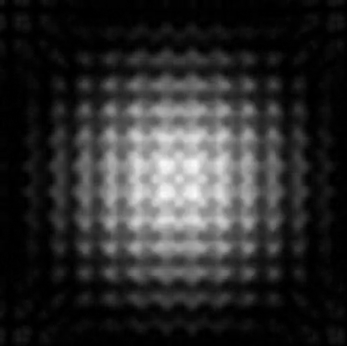
\includegraphics[width=5cm]{graphics/online_simulation.png}
    \caption{A screenshot of a "particle in a box" simulation found on Youtube}
\end{figure}

\newpage

\section{The mathematics of a particle in a box}
    \subsection{In one dimension}
        \subsubsection{Finding the Wave Function from Schrodinger's Equation}
        \label{sec:wave_equation_oned}
        The time dependent Schrodinger equation is given as:
        \begin{equation} \label{eq:time_dependant_equation}
            \left ( \frac{-\hbar^2}{2m} \nabla^2 + V \right ) \Psi(x,t)
            = i\hbar\frac{\partial}{\partial t}\Psi(x, t)   
        \end{equation}
        The time independent Schrodinger equation is given as:
        \begin{equation} \label{eq:time_independent_equation}
            \left ( \frac{-\hbar^2}{2m} \nabla^2 + V \right ) \Phi(x)
            = E \Phi(x)
        \end{equation}
        Where $\Psi$ is the wave equation. In terms of $\Phi$, $\Psi$ is
        denoted as:
        \begin{equation} \label{eq:dep_in_equation}
            \Psi(x, t) = e^{-i(E/\hbar)t}\Phi(x)
        \end{equation}
        Assuming the following is a solution to (\ref{eq:time_independent_equation}):
        \begin{equation} \label{eq:assumed_solution}
            \Phi(x) = A\cos(kx) + B\sin(kx)
        \end{equation}
        And given these two conditions that arise from the experiment:
        $$ \Phi(0) = \Phi(L) = 0 $$
        We plug them in the (\ref{eq:assumed_solution}) and find the following:
        \begin{align}
            \left\{\begin{matrix}
            A & = & 0 \\ 
            k & = & \frac{n}{L}\pi & \text{(n is the energy level)}
            \end{matrix}\right.
        \end{align}
        To find the value of $B$ we need to normalize the equation.\\
        The probability of finding the particle inside $[0; L]$ is $1$ because
        it cannot escape.
        \begin{align}
            \int_{0}^{L} |\Phi|^2 dx &= 1  \\
            B^2\int_{0}^{L} \sin^2\left ( \frac{n}{L}\pi x \right ) dx &= 1
        \end{align}
        And thus $B = \sqrt{\frac{2}{L}}$.\\
        Finally we get the solution to the time independent Schrodinger equation
        \begin{align}
            \Phi(x) = \sqrt{\frac{2}{L}}\sin(\frac{n}{L}\pi x)
        \end{align}

        \subsubsection{Energy at each quantum level $n$}
        \label{sec:energy_oned}
        We note the following
        \begin{align}
            \frac{\partial^2 }{\partial x^2} \Phi = -\left (
            \frac{n\pi}{L}\right )^2 \Phi
        \end{align}
        If we replace the results in (\ref{eq:time_independent_equation}) we find:
        $$ E_n = \frac{\hbar^2 n^2 \pi^2}{ 2 m L^2} $$
        Or simply:
        \begin{align*}
            E_n &= n^2 E_1 \\
            E_1 &= \frac{\hbar^2 \pi^2}{2 m L^2}
        \end{align*}

        \subsubsection{Probability function of the position}
        \label{sec:position_oned}
        The probability of finding the particle between $a$ and $b$ is the following:
        \begin{equation} \label{eq:probability_position}
            \left\{\begin{matrix}
            \int_{a}^{b} |\Phi|^2 dx & \text{if} \; \: a,b \in [0, L] \\ 
            0 & \text{otherwise}
            \end{matrix}\right.
        \end{equation}
        If we wish to find the position inside a box of width $\epsilon$ and
        center $a$ we would integrate between $a-\epsilon/2$ and $a+\epsilon/2$
        where both ends are between $0$ and $L$\\
        The integration will lead to the following:
        $$ P(x) = \frac{\epsilon}{L} + \frac{1}{2n\pi} \left [ 
            \sin\left ( \frac{2n\pi}{L}(a - \epsilon/2)\right ) -
            \sin\left ( \frac{2n\pi}{L}(a + \epsilon/2)\right )
        \right ]$$
        Which can be reduced more to the following form:
        $$ P(x) = \frac{\epsilon}{L} - \frac{1}{n\pi}\sin\left( \frac{n\pi}{L}\epsilon \right)
        \cos\left(\frac{2n\pi}{L}x\right)$$

    \subsection{In two dimensions}
        \subsubsection{The time-independent solution}
        This time we suppose the solution is
        \begin{equation} \label{eq:suppose_twod_solution}
            \Phi(x, y) = X(x)Y(y)
        \end{equation}
        \begin{align*}
            X(x) &= A\cos(k_x x) + B \sin(k_x x) \\
            Y(y) &= C\cos(k_y y) + D \sin(k_y y) \\
        \end{align*}
        Plugging (\ref{eq:suppose_twod_solution}) in (\ref{eq:time_independent_equation})
        and doing similar operations as \emph{~\ref{sec:wave_equation_oned}} we get
        the following solution:
        \begin{equation} \label{eq:twod_solution}
            \Phi(x, y) = \frac{2}{L} \sin\left( \frac{n_x\pi}{L}x\right)
                         \sin\left( \frac{n_y\pi}{L} y\right)
        \end{equation}

        \subsubsection{Energy in two dimensions}
        Doing the same steps as \emph{~\ref{sec:energy_oned}} we find that the energy has
        become:
        \begin{align}
            E_{n_x, n_y} &= \frac{\hbar^2 \pi^2}{2mL^2} (n^2_x + n^2_y)
        \end{align}
        Or simply:
        \begin{align*}
        E_{n_x, n_y} &= (n^2_x + n^2_y) \; E_{1,1} \\
        E_{1,1} &= \frac{\hbar^2 \pi^2}{2mL^2} 
        \end{align*}

        \subsubsection{Probability function of the position}
        Similar to section \emph{~\ref{sec:position_oned}} to find the
        probability of finding the particle inside the box of size
        $\epsilon$x$\epsilon$ we integrate the wave function inside a
        box of center $(x,y)$ and width $\epsilon$.
        $$ P(x, y) = \int^{y+\epsilon/2}_{y-\epsilon/2}\int^{x+\epsilon/2}_{x-\epsilon/2}
          |\Phi(x, y)|^2 dx dy $$
        After evaluating the integral we get the following function:
        \begin{equation} \label{eq:position_twod_equation}
            P(x, y) = \frac{1}{L^2} \; p(x) \; p(y)
        \end{equation}
        $$
        p(\alpha) = \epsilon - \frac{L}{n_\alpha\pi} \cos\left( \frac{2n_\alpha\pi}{L}\alpha \right)
        \sin\left( \frac{n_\alpha\pi}{L} \epsilon\right)
        $$

        \subsection{Generalizing the time-independent solution}
        The equation that we have found so far depends on two quantum numbers
        $n_x$ and $n_y$ and describes the particle for these energy levels only.
        However the final time-dependant equation is a combination of many of these
        equations. The final time-independent equation is:
        \begin{equation} \label{eq:general_position}
            \Phi(x,y) = \sum_{n} c_n \Phi_{n_x, n_y}(x,y)
        \end{equation}
        Where the constant $c_n$ is the square root of the probability of getting
        the equation $\Phi_{n_x, n_y}$ that describes the particle in the box.

        \subsection{Generalizing the probability function}
        Since we have a more general wave function we need to have a more general
        probability function for the position. The new definition is generated from
        integrating $\Phi$ between $a-\epsilon/2$ and $a+\epsilon/2$. The result is:
        $$ P(x, y) = \sum_{n} c^2_n \: P_n(x, y)$$

\newpage

\section{Implementation}
    \subsection{Synopsis}
    This simulation will display the probability of finding the particle in sub-boxes in the box
    as well as display the energy in the sub-box of width $\epsilon$. Each frame displays the
    particle with a new set of probabilities for each energy level.\\\\
    The probability of the position will be visualized by the intensity of the color. The brighter
    the color, the higher the probability.\\\\
    The energy however will be visualized using the standard colors assigned to energies; lower
    energies have blue-shades while high energies have red-shades.

    \subsection{Conventions}
    Some of the conventions adopted throughout the code are
    \begin{itemize}
        \item words in functions, structs and variable names are separated by an \_ (underscore)
        \item CUDA kernels start with the keyword \texttt{cuda\_}.\\
              For example \texttt{cuda\_probability}
        \item CUDA device functions start with \texttt{cuda\_} and end with \texttt{\_device}.\\
              For example \texttt{cuda\_probability\_1d\_device}
        \item Tiny mathematical and physical constants, such as $\hbar$ are expressed
              as float numbers without their orders.\\ For example $\hbar = 1.054\cdot10^{-34}$
              is defined as \texttt{\#define HBAR 1.054}
    \end{itemize}

    \subsection{Brightness and Color mapping}
        \subsubsection{Brightness} \label{sec:brightness}
        \label{sec:brightness}
        The intensity of the colors denote the probability of finding the particle. Since
        probabilities are always between 0 and 1, converting them to intensities is just
        a matter of mapping the probabilities from $[0, 1]$ to $[0, 255]$.\\\\
        However $\epsilon$ is a small number, so the probability is always small; usually
        less than $0.1\%$. Therefore we need to find the highest probability in the space
        and remap from $[0, \text{max}]$ to $[0, 255]$. At first I have tried to brute force
        the problem exploiting my GPU using functions to find maximums using reduction. But
        the process of finding the highest probability of a particle with 10 energy levels
        inside a box divided into 262,144 boxes took around 28ms. Allowing me to get only
        35fps in the animation.\\
        A new solution needed to be adopted and I went over the equations again to try and
        find that maximum analytically. My results are:\\\\
        For $p(\alpha)$ to be maximal
        $$\frac{\epsilon}{L} - \frac{1}{n_{\alpha}\pi} \sin\left(\frac{n_{\alpha}\pi}{L}\epsilon\right)
        \cos\left(2\frac{n_{\alpha}\pi}{L}\alpha\right)$$
        needs to be maximal.  And this is achieved when $\cos{x} = -1$ which is possible
        since $0 \leq x \leq 2\pi$. Therefore the highest probability for one energy
        level is: 
        $$\frac{\epsilon}{L} + \frac{1}{n_{\alpha}\pi} \sin(\frac{n_{\alpha}\pi}{L}\epsilon)$$
        Following similar analysis we can deduce that the highest probability (denoted by
        $m$) is close to,
        but not exactly:
        $$m = m_x . m_y$$
        $$m_{\alpha} = \frac{\epsilon}{L} + \sum_i \left ( c^2_i \frac{1}{n_{\alpha_i}\pi}
        \sin\left(\frac{n_{\alpha_i}\pi}{L}\epsilon\right) \right )$$\\\\
        \textbf{UPDATE} After implementing and testing the algorithm the uncertainty in the algorithm
        has proved to be overwhelming and the probabilities' range was no longer $[0, 1]$ but much smaller.
        Therefore a fallback was needed.\\\\
        The approach followed was a bruteforce solution where we compute the probabilities at each at each
        pixel and search for the largest. However to make the searching faster a reduction algorithm
        was adopted to speed it up. The algorithm creates a much smaller array in which it stores
        the maximum of a chunk of the original array. Then on the CPU we loop over the results (which are
        usually 32) and pick the maximum of these. The following illustration describes how the maximum
        reduction algorithm works
        \begin{figure}[hb]
            \label{fig:reduction}
            \centering
                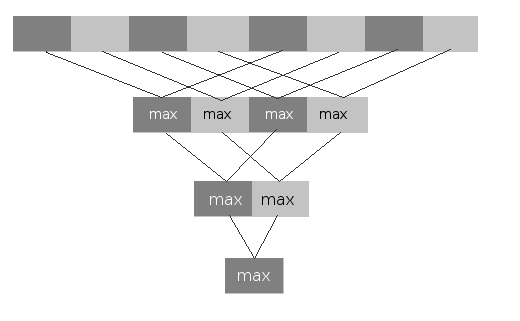
\includegraphics[width=8cm]{graphics/max_reduction.png}
            \caption{Finding the maximum element in an array using reduction}
        \end{figure}
        The fact that this algorithm was used adds a restriction on the dimensions of the window. The height
        and the width of the window need to be a power of 2 for this algorithm to work effectively.
        No solution has been made up yet to generalize the dimensions of the window.
        
        \subsubsection{Tint and Color}\label{sec:colormap}
        The tint in the color represents the energy of the particle. Red is the highest
        energy and blue is the lowest. If we can map the energy in an interval between
        0 and 1 we can easily get the RGB values. The following equation can be applied
        $$ \begin{bmatrix} R_{xy} \\ G_{xy} \\ B_{xy} \end{bmatrix} = P(x, y)
        \begin{bmatrix} 255E \\ 20 \\ 255(1-E) \end{bmatrix} $$
        Where $P(x, y)$ is the probability of finding the particle at $(x, y)$ and between
        0 and 1. And $E$ is the energy remapped between 0 and 1. \\\\
        To problem of remapping the energy is easy to solve. Through mathematical analysis
        we can show that the highest energy we can find is
        $$ E_{max} = (n^2_{max_x} + n^2_{max_y})\frac{\hbar^2\pi^2}{2mL^2} $$
        And therefore we can remap any energy we find to a value in the interval $[0, 1]$
        and find the corresponding RGB values.

        \subsection{Next set of probabilities}
        \label{sec:nextproba}
        Every frame in the animation consists of a new set of probabilities close to the ones of the
        previous frame. A problem came up and that is how to generate new set of probabilities close
        to the ones in the previous frame to insure the smooth animation between the frames.\\\\
        The model adopted to insure the smoothness and the continuity in the probabilities consists
        of multiple sine waves where the period of one is 10 times more than its neighbor and so on.
        If plotted, the model looks like the following: (the sines were stretched vertically for a better
        visualization)
        \begin{figure}[hb]
            \centering
                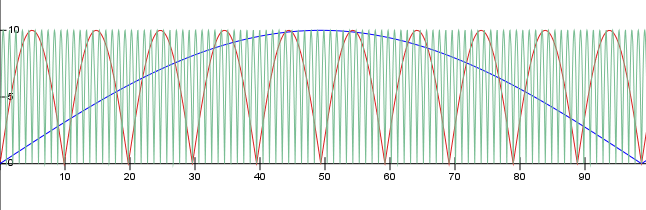
\includegraphics[width=8cm]{graphics/sine_probabilities.png}
            \caption{Plotting
               $x(t) = 10\left| sin \left( \frac{0.1}{\pi}t \right) \right|$, 
               $y(t) = 10\left| sin \left( \frac{1}{\pi}t \right) \right|$, 
               $z(t) = 10\left| sin \left( \frac{10}{\pi}t \right) \right|$}
        \end{figure}
        After finding the values of each sine wave at a time $t$ we can normalize the answers so that
        their sum is $1$. Bellow is a table representing some values normalized.
        \begin{center}
            \begin{tabular}{| c | c | c | c |}
                \hline
                \textbf{Time} & \textbf{x} & \textbf{y} & \textbf{z} \\ \hline
                0.1 & 0.0091 & 0.0915 & 0.8994 \\
                0.2 & 0.0096 & 0.0957 & 0.8947 \\
                0.3 & 0.0104 & 0.1035 & 0.8861 \\
                0.4 & 0.0116 & 0.1159 & 0.8725 \\
                0.5 & 0.0136 & 0.1350 & 0.8515 \\
                0.6 & 0.0166 & 0.1648 & 0.8186 \\
                0.7 & 0.0215 & 0.2135 & 0.7649 \\
                0.8 & 0.0304 & 0.3006 & 0.6690 \\
                0.9 & 0.0490 & 0.4834 & 0.4675 \\
                1.0 & 0.0824 & 0.8102 & 0.1074 \\
                1.1 & 0.0479 & 0.4698 & 0.4822 \\
                1.2 & 0.0368 & 0.3590 & 0.6042 \\
                1.3 & 0.0322 & 0.3134 & 0.6544 \\
                1.4 & 0.0309 & 0.2987 & 0.6704 \\
                1.5 & 0.0317 & 0.3053 & 0.6630 \\
                1.6 & 0.0347 & 0.3324 & 0.6329 \\
                1.7 & 0.0405 & 0.3859 & 0.5736 \\
                1.8 & 0.0509 & 0.4818 & 0.4673 \\
                1.9 & 0.0701 & 0.6595 & 0.2704 \\
                2.0 & 0.0859 & 0.8022 & 0.1119 \\ \hline
            \end{tabular}
        \end{center}
        \begin{center}Table 1: Values from $x(t)$, $y(t)$ and $z(t)$ at different times\end{center}
        A general formula can be deduced to find the equation of the nth wave.
        \begin{align}
            P_{n}(t) = \left| sin\left( \frac{10^{1-n}}{\pi}t \right)\right|
        \end{align}

    \subsection{(G)UI}
    The GUI will be farely simple, a window where the simulation is drawn on. The user can
    control the simulation by keystrokes listed bellow.
    \begin{center}
        \begin{tabular}{|r|r|}
        \hline
            . & Increase the time offset \\ \hline
            , & Decrease the time offset \\ \hline
            SPACE & Toggle pausing \\ \hline
            0 & Reset the animate (t = 0) \\ \hline
            ESC & Quit the simulation \\ \hline
        \end{tabular}
    \end{center}
    As well, the user can control the number of wave functions that are being simulated using
    command line arguments as follow
    \begin{verbatim}pbox n\end{verbatim}
    Where \verb|n| is the number of wave functions the user wishes to simulate.

\newpage
\section{API}
    \subsection{Structures}
        \subsubsection{particle}
        {\bf Members}
        \begin{itemize}
            \item \begin{verbatim}float mass\end{verbatim} The mass of the particle.
            \item \begin{verbatim}int energy_levels\end{verbatim} The number
                  of energy levels the particle has, i.e. the number of wave
                  functions that describe the particle.
            \item \begin{verbatim}float *particles\end{verbatim} The
                  probabilities of each wave function. The length of the array
                  this variable points to should be \verb|energy_levels|.
        \end{itemize}

    \vspace{1cm}
    \subsection{Global Variables}
    The program uses these global variables
    \begin{itemize}
        \item \verb|cudaGraphicsResource *resource|\\\mar- The graphics resource that is
              linked to the OpenGL environment.
        \item \verb|GLuint buffer|\\\mar- The buffer used by OpenGL.
        \item \verb|float INCREASE_TIME|\\\mar- The time offset used to increase the time
              between the frames.
        \item \verb|particle p|\\\mar- The particle that the program is about.
        \item \verb|float t|\\\mar- The current time (set as the offset).
        \item \verb|int frames|\\\mar- The number of frames.
        \item \verb|float total_time|\\\mar- The total time.
        \item \verb|int PAUSE|\\\mar- Whether the animation is paused.
    \end{itemize}

    \newpage
    \subsection{Functions}
        \vspace{1cm}
        \subsubsection{float max(float *numbers, int N)}
        This function finds the maximum number in an array of numbers using reduction
        as described in ~\ref{fig:reduction}.\\
        \\{\bf Parameters}\\
        \verb|float *numbers|\\\mar- A pointer of the array to find the maximum of.\\
        \verb|int N|\\\mar- The length of \verb|numbers|. {\bf Should be a power of 2}.\\
        \\{\bf Returns}\\
        \verb|float|, the maximum number in the array.

        \vspace{1cm}
        \subsubsection{void next\_probabilities(float t, int N, float *probabilities)}
        This function generates a new set of probabilities as described in ~\ref{sec:nextproba}.
        \\\\{\bf Parameters}\\
        \verb|float t|\\\mar- The time parameter required in the algorithm.\\
        \verb|int N|\\\mar- the number of parameters to generate, i.e. the length of
        the next parameter.\\
        \verb|float *probabilities|\\\mar- The array to write the new probabilities to.

        \vspace{1cm}
        \subsubsection{void create\_particle(particle *p, int N, float mass)}
        This function creates a new particle.\\
        \\{\bf Parameters}\\
        \verb|particle *p|\\\mar- The particle to store the new particle in.\\
        \verb|int N|\\\mar- The number of wave functions (energy levels) that describe
        the particle.\\
        \verb|float mass|\\\mar- The mass of the particle

        \vspace{1cm}
        \subsubsection{float probability(particle *p, float x, float y)}
        This function finds the probability of finding a particle inside a box of center
        $(x, y)$ and of width and height $\epsilon$.\\
        \\{\bf Parameters}\\
        \verb|particle *p|\\\mar- The particle to act on\\
        \verb|float x|\\\mar- The x-coordinate of the particle\\
        \verb|float y|\\\mar- The y-coordinate of the particle\\
        \\{\bf Returns}\\
        \verb|float|, the probability of finding the particle at $(x, y)$

        \vspace{1cm}
        \subsubsection{float max\_probability(particle *p)}
        This function finds the highest probability of existing at a position $(x, y)$
        in the space, i.e. inside the box. The function is used to later on map the
        probabilities from $[0, \text{max}]$ to $[0, 255]$ for color-brightness purposes.
        The algorithm adopted is described in ~\ref{sec:brightness}.\\
        \\{\bf Parameters}\\
        \verb|particle *p|\\\mar- The particle to find the highest probability of existing\\
        \\{\bf Returns}\\
        \verb|float|, the highest probability to exist.

        \vspace{1cm}
        \subsubsection{void initGL(int *argc, char **argv)}
        This function initializes the OpenGL environment.\\
        \\{\bf Parameters}\\
        \verb|int *argc|\\\mar- The length of the next parameter.\\
        \verb|char **argv|\\\mar- The parameters supplied to the OpenGL environment.
        
        \vspace{1cm}
        \subsubsection{void display()}
        This function takes care of drawing the output on the canvas on every iteration.
        As well it prints out the current time, the average time per frame in milliseconds
        and the offset that is used to increase the time.

        \vspace{1cm}
        \subsubsection{void key(unsigned char k, int x, int y)}
        This function manages the keystrokes in the canvas.\\
        \\{\bf Parameters}\\
        \verb|unsigned char k|\\\mar- The character pressed.\\
        \verb|int x|\\\mar- The x-coordinate where the character is pressed.\\
        \verb|int y|\\\mar- The y-coordinate where the character is pressed.

        \vspace{1cm}
        \subsubsection{void free\_resources()}
        This function is used to clean after closing the window, i.e. free the resources.

        \vspace{1cm}
        \subsubsection{void createVBO(GLUint *buffer, cudaGraphicsResource **resource,
            unsigned int flags)}
        This function initializes the buffer and the resources that are used by OpenGL.\\
        \\{\bf Parameters}\\
        \verb|GLuint *buffer|\\\mar- The buffer used by OpenGL.\\
        \verb|cudaGraphicsResource **resource|\\\mar- The CUDA resource to link to the buffer\\
        \verb|unsigned int flags|\\\mar- The flags used by OpenGL.

        \vspace{1cm}
        \subsubsection{void launch\_kernel(uchar4 *pos)}
        This function launches the kernel that fills the CUDA resource which will be used
        to draw on the canvas.\\
        \\{\bf Parameters}\\
        \verb|uchar4 *pos|\\\mar- The array of pixel data

        \vspace{1cm}
        \subsubsection{void runCuda(cudaGraphicsResource **resource)}
        This function creates the resources for the kernel and launches it.\\
        \\{\bf Parameters}\\
        \verb|cudaGraphicsResource **resource|\\\mar- The CUDA resource.

        \vspace{1cm}
        \subsubsection{void run(int argc, char **argv)}
        This function runs everything, i.e. initializes the environment, selects
        a valid GPU card, creates the resources and launches the GUI.\\
        \\{\bf Parameters}\\
        \verb|int argc| the length of the next parameter.\\
        \verb|char **argc| the parameters used by the OpenGL environment.\\

        \vspace{1cm}
        \subsubsection{void usage(char* program\_name)}
        This function prints out the help message.\\
        \\{\bf Parameters}\\
        \verb|char* program_name|\\\mar- The name of the program to run
    
    \newpage
    \subsection{CUDA Kernels}
        \vspace{1cm}
        \subsubsection{\_\_global\_\_ void cuda\_max(float *numbers, int N, float *partialMax)}
        This kernel finds the maximum in buckets (sub-array) of the numbers array and
        fills the partialMax array using the reduction method described in ~\ref{fig:reduction}.
        \\\\{\bf Parameters}\\
        \verb|float *numbers|\\\mar- The numbers to find the maximum of.\\
        \verb|int N|\\\mar- The length of the array of numbers.\\
        \verb|float *partialMax|\\\mar- The list containing the maximum of the buckets.

        \vspace{1cm}
        \subsubsection{\_\_global\_\_ void cuda\_probability\_to\_map(float *probabilities, int n,
        float *map)}
        This kernel maps the coordinate array to the probability array.\\
        \\{\bf Parameters}\\
        \verb|float *probabilities|\\\mar- The probability set of each wave function.\\
        \verb|int n|\\\mar- The number of wave functions.\\
        \verb|float *map|\\\mar- The array that will be filled with probabilities

        \vspace{1cm}
        \subsubsection{\_\_global\_\_ void cuda\_probability(float *p, in N, float x, float y,
        float *probability)}
        This kernel finds the probability of finding the particle in a certain position.\\
        \\{\bf Parameters}\\
        \verb|float *p|\\\mar- The probability set of each wave function.\\
        \verb|int N|\\\mar- The number of energy levels.\\
        \verb|float x|\\\mar- The x-coordinate of the particle.\\
        \verb|float y|\\\mar- The y-coordinate of the particle.\\
        \verb|float *probability|\\\mar- The variable to write the probability to.

        \vspace{1cm}
        \subsubsection{\_\_global\_\_ void kernel(uchar4 *ptr, float *probabilities, int N,
        float max\_proba)}
        This kernel fills the pixel array with the corresponding colors to display them.\\
        \\{\bf Parameters}\\
        \verb|uchar4 *ptr|\\\mar- The array of pixels\\
        \verb|float *probabilities|\\\mar- The array of probabilities of each wave function.\\
        \verb|int N|\\\mar- The number of wave functions.\\
        \verb|gloat max_proba|\\\mar- The highest probability in the space.

    \newpage
    \subsection{CUDA Device Functions}
        \vspace{1cm}
        \subsubsection{\_\_device\_\_ float cuda\_probability\_1d\_device(int n, float x)}
        This function finds the probability of finding the particle in one dimension 
        at the position x and at the energy level n.\\
        \\{\bf Parameters}\\
        \verb|int n|\\\mar- The energy level of the particle\\
        \verb|float x|\\\mar- The position of the particle\\
        \\{\bf Returns}\\
        \verb|float|, the probability.

        \vspace{1cm}
        \subsubsection{\_\_device\_\_ float cuda\_probability\_1d\_device(float *probabilities,
        int n, float x, float y)}
        This function finds the probability of finding the particle at a fixed position
        given a set of probabilities, the number of energy levels and the position.\\
        \\{\bf Parameters}\\
        \verb|float *probability|\\\mar- The probability of each energy level.\\
        \verb|int n|\\\mar- The number of energy levels.\\
        \verb|float x|\\\mar- The x-coordinate of the particle.\\
        \verb|float y|\\\mar- The y-coordinate of the particle.\\
        \\{\bf Returns}\\
        \verb|float|, the probability.

        \vspace{1cm}
        \subsubsection{\_\_device\_\_ float energy(float mass, int n)}
        This function finds the energy of the particle at a precise energy level.\\
        \\{\bf Parameters}\\
        \verb|float mass|\\\mar- The mass of the particle.\\
        \verb|int n|\\\mar- The energy level the particle is at.\\
        \\{\bf Returns}\\
        \verb|float|, the energy at the energy level n.

        \vspace{1cm}
        \subsubsection{\_\_device float highest\_energy(float mass, int n)}
        This function finds the highest energy the particle can reach. This function
        is used for color mapping described in ~\ref{sec:colormap}.\\
        \\{\bf Parameters}\\
        \verb|float mass|\\\mar- The mass of the particle.\\
        \verb|int n|\\\mar- The highest energy level the particle can reach.\\
        \\{\bf Returns}\\
        \verb|float|, the highest energy

\newpage
\section{Results}
    \subsection{Screenshots}
    These are some screenshots taken from the simulation. Only 5 wave functions are illustrated.\\
    \begin{table}[ht]
        \begin{center}
        \begin{tabular}{c c c}
            
\includegraphics[width=3.5cm]{graphics/result1.png} &
            
\includegraphics[width=3.5cm]{graphics/result3.png} &
            
\includegraphics[width=3.5cm]{graphics/result2.png} \\
            1 & 2 & 3 \\\\
            
\includegraphics[width=3.5cm]{graphics/result6.png} &
            
\includegraphics[width=3.5cm]{graphics/result4.png} &
            
\includegraphics[width=3.5cm]{graphics/result5.png} \\
            4 & 5 & 6
        \end{tabular}
        \end{center}
    \end{table}\\
    From observing the screenshots we can generate a table that encapsulate the wave functions most visible
    in the screenshots
    \begin{table}[ht]
        \begin{center}
            \begin{tabular}{| r | c | c | c | c | c |}
            \hline
            Screenshot & 1 & 2 & 3 & 4 & 5 \\ \hline
            1 & $\times$ & $\times$ & & & \\ \hline
            2 & $\times$ & $\times$ & $\times$ & & $\times$ \\ \hline
            3 & & $\times$ & $\times$ & $\times$ & \\ \hline
            4 & & $\times$ & $\times$ & & $\times$ \\ \hline
            5 & & & $\times$ & & $\times$ \\ \hline
            6 & $\times$ & & & & $\times$ \\ \hline
            \end{tabular}
        \end{center}
    \end{table}

    \subsection{Benefits}
    Thanks to this simulation the problem of the Particle in a box is now much clearer
    to me, and I was able to understand more about the topic.\\\\
    As well it helped me visualize another problem related and that is \emph{Heisenberg's
    Uncertainty Principle} described mathematically as $\delta_x\delta_p \geq \frac{\hbar}{2}$.
    As described in section ~\ref{sec:brightness} the more intense the color at a pixel is,
    the higher the probability. For higher the quantum number is the larger the energy, and
    since the energy is directly related to the momentum of the particle we should expect
    a large uncertainty in the position of the particle. That is perfectly illustrated in this
    simulation, as the graphics become red the higher the energy is and we can see numerous
    bright spots on the canvas, meaning there is a high probability for the particle to exist
    in many positions, therefore agreeing with Heisenberg's Uncertainty Principle.

\newpage
\section{Code License: GNU General Public License}
Copyright (C) 2013 George Zakhour\\

This program is free software: you can redistribute it and/or modify it under
the terms of the GNU General Public License as published by the Free Software
Foundation, either version 3 of the License, or (at your option) any later
version.\\

This program is distributed in the hope that it will be useful, but WITHOUT ANY
WARRANTY; without even the implied warranty of MERCHANTABILITY or FITNESS FOR A
PARTICULAR PURPOSE. See the GNU General Public License for more details.\\

You should have received a copy of the GNU General Public License along with
this program. If not, see http://www.gnu.org/licenses/.\\


\end{document}
